\section{Theoretical background}
\label{sec:theory}

\subsection{Beginnings of quantum mechanical wave dynamics}

In this section, we would like to give a brief introduction to the theory of \acrshort{qm}. In this summary of physics history, we rely mainly on Tamás Geszti's \acrshort{qm} book \cite{geszti2007}.
For English literature, we would like to point the reader's attention towards the critically acclaimed book of Claude Cohen-Tannoudji et al. \cite{tannoudjiVol1}.
%We will start our introduction with Max Planck.
%He gave an explanation for the drop in the spectrum of black-body radiation for high frequencies with constant temperature.
%He argued that each harmonic oscillator can only obtain energy in discrete energy elements of
%\begin{equation}
%	\label{eq:energy_quantum}
%	E_\delta = h\nu
%\end{equation}
%where $h$ is called the Planck constant and equals to $h = 6,6 \times 10^{-34}\;Js$
%and $\nu$ is the frequency of the oscillator.
%For convenience physicists tend to use $\hbar = \frac{h}{2\pi}$ reduced Planck constant.
%With this equation \ref{eq:energy_quantum} can be written in the form of
%\begin{equation}
%	E_\delta = \hbar\omega
%\end{equation}
%
%At this point, it was known to physicists that a black body can be modeled with electromagnetic harmonic oscillators with different modes that satisfy the boundary conditions of the box. Consequently, Planck was able to give a formula that accurately models the energy emission of black-bodies.
%The next advancement was in 1905, when Albert Einstein explained the photoelectric experiment.
%This experiment was first performed and documented by Fülöp Lénárd resulting in a Nobel prize for him.
%This experiment demonstrates that electrons can exit a metal electrode only by shining light on it.
%Here an important observation was made, which can be described by saying that the $E_{photo}$ energy of exited electron only depends on the color of light shining on the electrode.
%Einsteins discovery can be formally written in the following equation
%\begin{equation}
%	E_{photo} = h\nu - W
%\end{equation}
%where $W$ is the work required for the electron to leave the electrode.
%This is the second time the Planck constant appears in a physical formula.
%It suggests that the electron absorbs the energy of one single light quantum (photon, as we would call today).
%
%Ernest Rutherford experimented with shooting high energy positively charged $\alpha$-particles into materials and observing the refraction of these particles.
%He came to the conclusion that the largest portion of the mass of the materials is clumped into heavy positively charged cores and light negatively charged electrons surround the positive cores.
%According to his explanation the reason why these negatively charged particles do not fall into the positive core is that they orbit the core similarly to how planets do orbit the Sun.
%This however results in a paradox.
%Negatively charged orbiting particles should emit electromagnetic radiation thus quickly loosing energy and consequently falling into the core.
%
%Physicist have examined the color spectrum of atomic gases such as hydrogen.
%They observed that such gases exhibit a spectrum of discrete lines.
%To explain this strange phenomena in 1913, Niels Bohr made the connection between Planck's energy quantum hypothesis and Einstein's photon hypothesis.
%He stated that the electrons orbiting the atomic core occupy only orbitals with certain energy levels, and somehow evade the continuous transition between these orbitals.
%When they do make the transition between the discrete energy levels of $E_n$ and $E_m$ they emit or absorb photons based on whether they gained or lost energy.
%\begin{equation}
%	h\nu = E_m - E_n
%\end{equation}


In 1924, Louis de Broglie recognized that an electron moving with momentum of $p=M_ev$ can also be thought of as the propagation of some kind of a matter wave with $\lambda$ wavelength.
\begin{equation}
	\label{eq:de_broglie}
	\lambda = \frac{h}{p}
\end{equation}
where $h$ is called the Planck constant and equals to $h = 6,6 \times 10^{-34}\;Js$.
This also explains the discrete energy levels in Bohr's model.
The allowed orbitals are those where the wave is a single-valued function and thus closes into itself after one full rotation of $2\pi$ radians.
If we use polar coordinates, this means that the wave has the same complex amplitude for coordinates $\alpha$ and $\alpha + n2\pi$ where $n = 0, 1, 2, \dots$.
Here we can further modify equation \ref{eq:de_broglie} and arrive to
\begin{equation}
	\vec{p} = \hbar \vec{k}
\end{equation}
where $\vec{k}$ is the wave vector and $\hbar = \frac{h}{2\pi}$ is the reduced Planck constant.
The amplitude of this vector equals $\|\vec{k}\|= \frac{2\pi}{\lambda}$, and its direction is perpendicular to the wavefront.

Experiments show that matter waves exhibit self-interfering behavior similar to electromagnetic waves\footnote{An electron always only interferes with itself while light waves coming from multiple light sources can also interfere with each other.}.
For example, the double-slit experiment, where a wave propagates through a barrier with a pair of two narrow slits and consequently creates an interference pattern on a canvas placed after the barrier, can be performed not only with light but a single electron as well.
When the experiment is performed with electrons, the canvas is replaced with a measurement device that is able to register the incoming electron.
By performing this experiment once, the measuring device will only register the electron at a single location.
The interference becomes noticeable only after repeating the measurement multiple times since the distribution of the measured electron impact locations converges to the interference pattern.
This behavior is also referred to as wave–particle duality because the particle interferes with itself, but also, there is only one single impact at the measuring device for each iteration of the experiment.
Another important experimental observation is that if we create the linear combination of multiple matter waves and then the combined wave evolves over time than the resulting wave is precisely the same as if the originally combined waves would have evolved independently and we would only have combined the resulting waves.
This latter property was also true for electromagnetic waves, and its called the superposition principle.
Please note that although we keep comparing electromagnetic waves with matter waves, the two are different phenomena.
One significant difference is that interference of electromagnetic waves happen due to different strength of electric and magnetic fields.
In \acrshort{qm} the wave function has a complex value thus, it can interfere even when only the phase is different and the amplitude is the same.
Our goal in emphasizing the similarities is only to reinforce a possible intuition in those perhaps more familiar with the world of electromagnetism.

\subsection{Wave packet dynamics}

Erwin Schrödinger introduced the concept of the \acrfull{wp} to show that in limiting cases \acrshort{qm} gives back the classical particle model where small bullets are moving around and colliding.
This particle-like propagation of a \acrshort{wp} of the wave is due to the superposition of waves with different frequencies forming peaks.
These waves extinguish each other for the most part, but at some position and time coordinates, the amplitudes add up to larger amplitude.
An example of this is demonstrated in figure \ref{fig:superposition}.
\begin{figure}[hbt!]
	\centering
	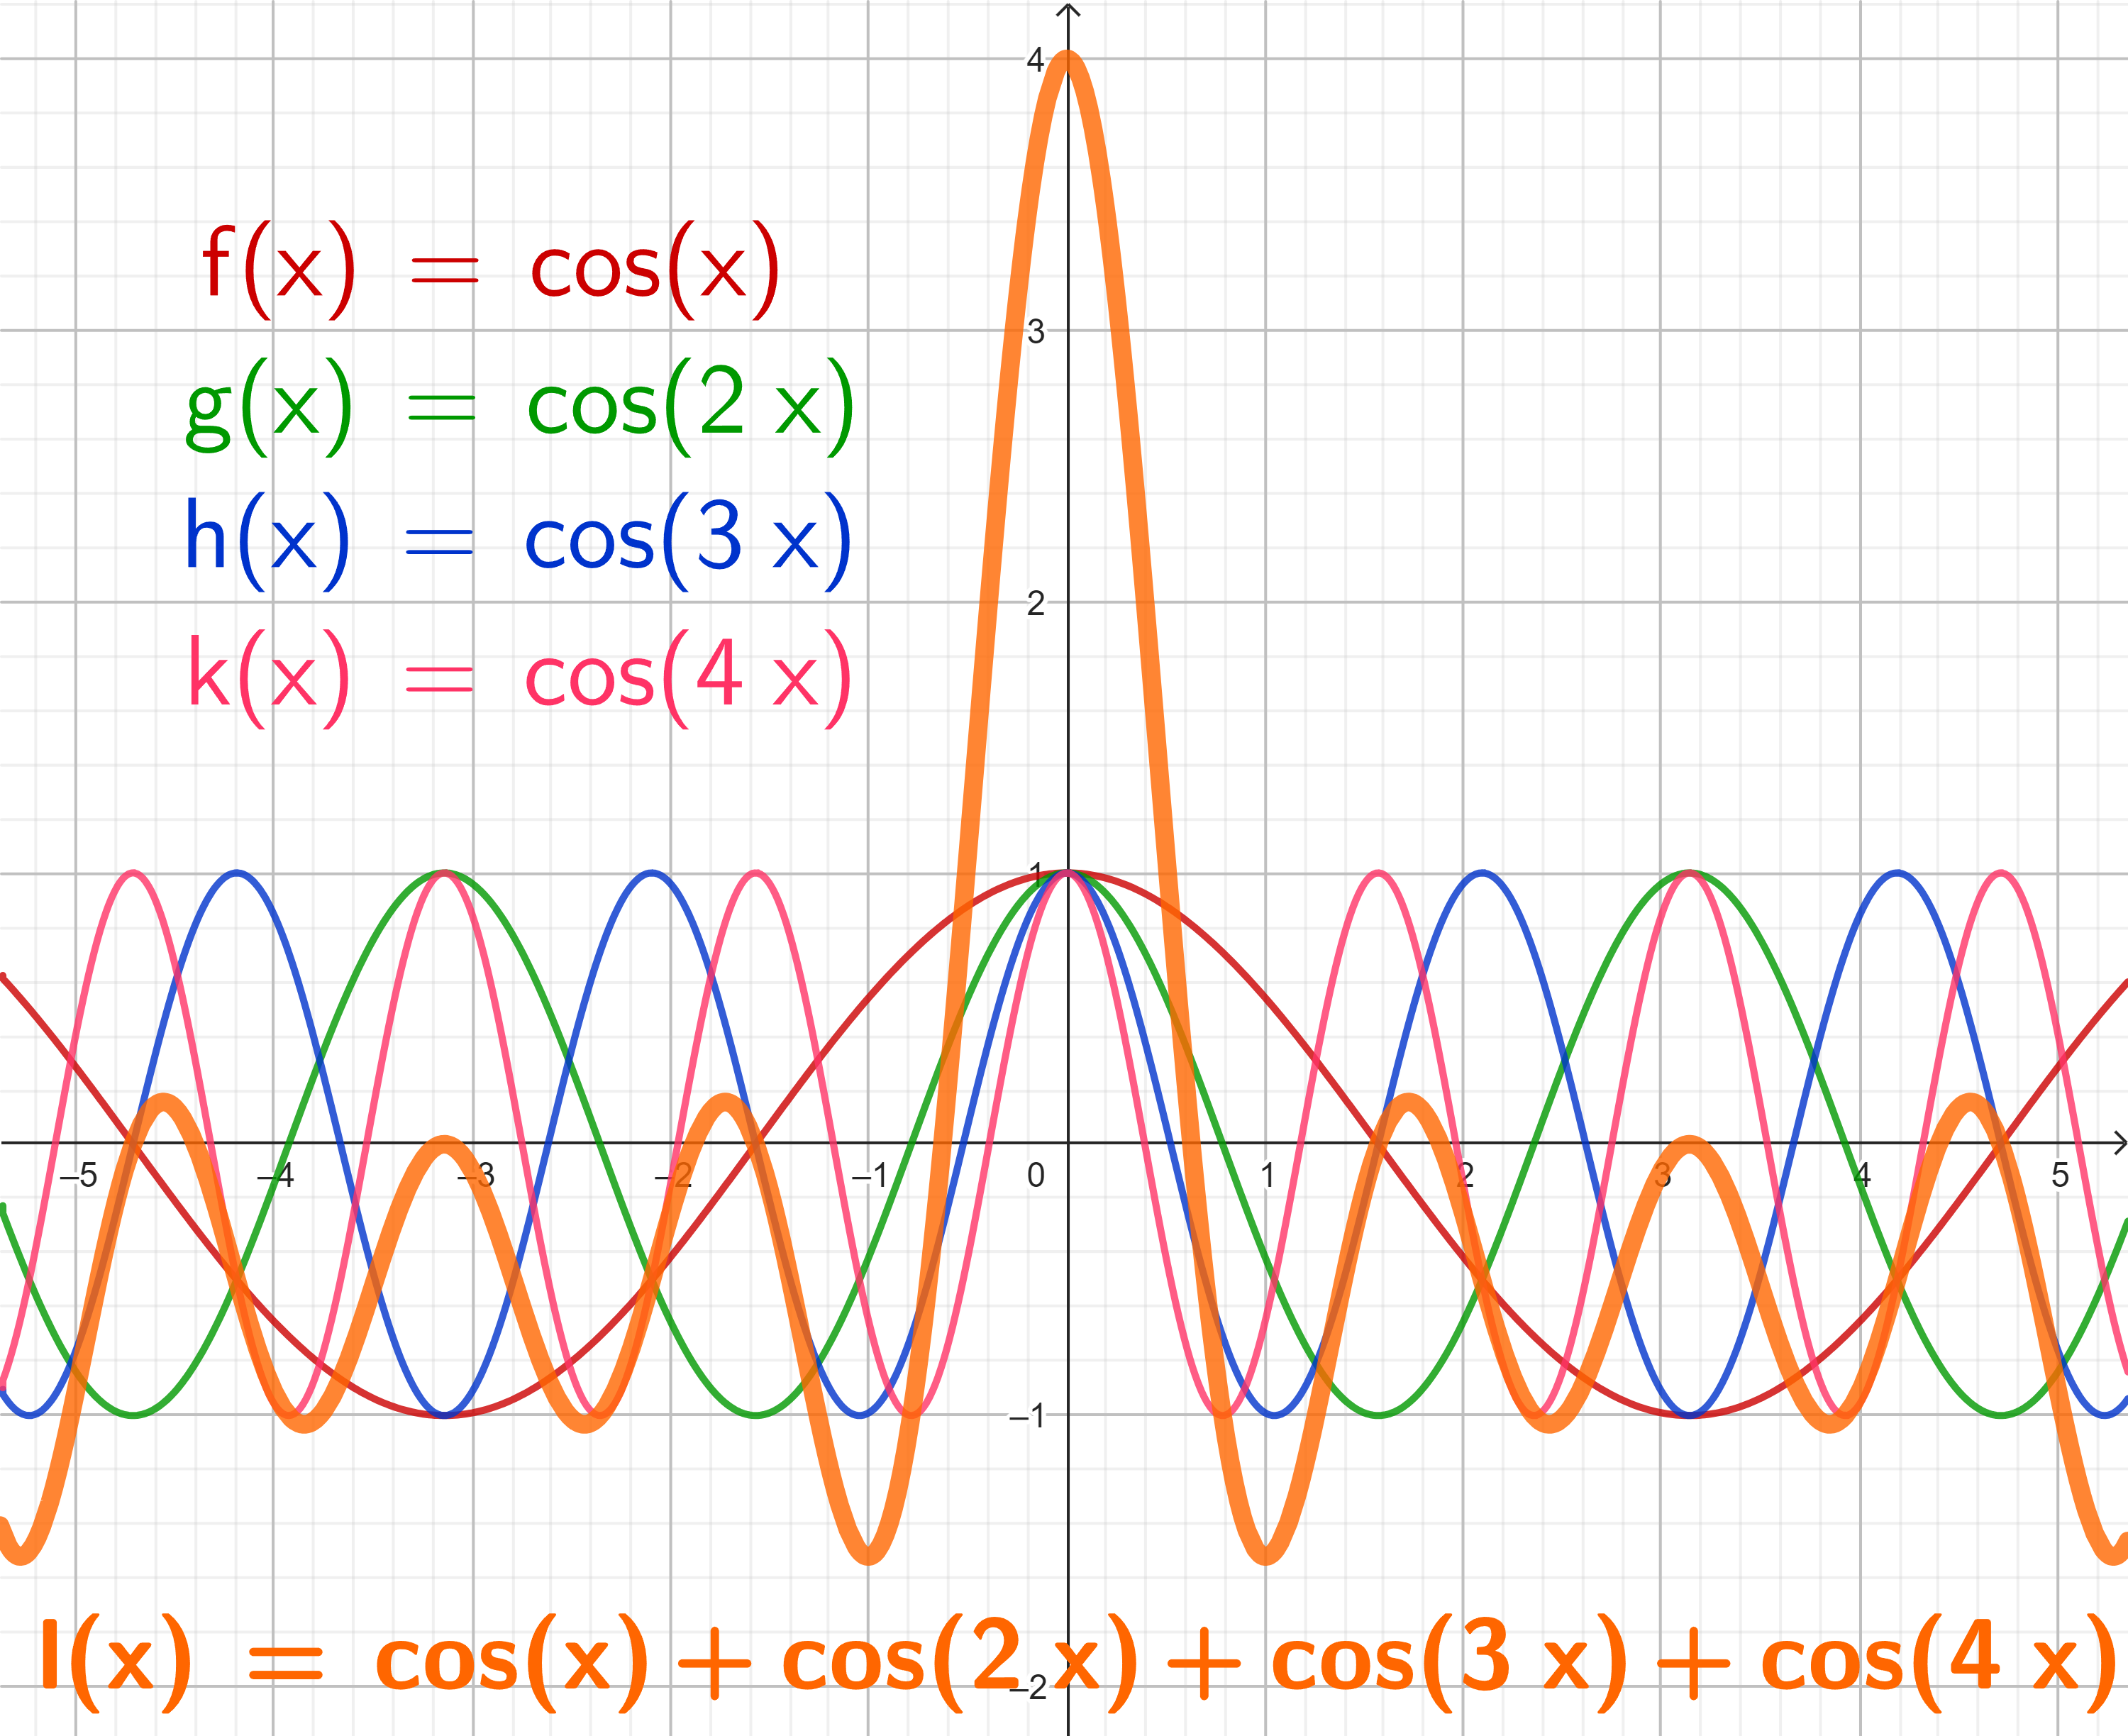
\includegraphics[width=0.5\textwidth]{figures/Superposition of cosine waves.png}
	\caption{Superposition of cosine waves with different wavelength: the superposition forms a peak at the $x = 0$ coordinate}
	\label{fig:superposition}
\end{figure}

$\Psi_k$ denotes the complex amplitude of a matter wave with $k=\frac{2\pi}{\lambda}$ wave number. The formula of a plane wave propagating in positive $x$ direction can be described in the form of equation \ref{eq:plane_wave_k}.

\begin{equation}
	\label{eq:plane_wave_k}
	\Psi_k(x, t) = e^{i(kx - \omega t)}
\end{equation}

Let's calculate the superposition of waves with different wave numbers! We assume that the angular velocity $omega(k)$ depends on the $k$ wave number and that the waves with different wave numbers have various $c(k)$ weights in the linear combination. This gives the following Fourier integral:
\begin{equation}
	\label{eq:combination_of_waves}
	\Psi(x, t) = \int_k c(k) sin[kx - \omega(k)t]\; dk
\end{equation}

By analyzing this formula, we can determine the propagation velocity of the amplitude peaks.
In equation \ref{eq:combination_of_waves}, the peaks form where and when the phase of the sine function is not dependent on the $k$ integration variable. In other words, the derivative of the phase with respect to $k$ is zero.
\begin{equation}
	\label{eq:derivative_of_phase}
	\frac{d}{dk}[kx - \omega(k)t] = x - \frac{d}{dk}\omega(k)t = 0
\end{equation}

By generalizing for all spatial coordinates and rearranging equation \ref{eq:derivative_of_phase}, we get the group velocity of the wave.
\begin{equation}
	\label{eq:group_velocity}
	\vec{v}_{group} = \frac{\delta \omega(\vec{k})}{\delta \vec{k}}
\end{equation}
By using the $E := \hbar \omega$ and $\hbar \vec{k} = \vec{p}$ substitutions for the energy and momentum, we arrive at the classically known formula for a particle of mass $m$
\begin{equation}
	\label{eq:classical_group_velocity}
	\vec{v}_{group} = \frac{\delta E(\vec{p}, \vec{r})}{\delta\vec{p}} = \frac{\delta}{\delta\vec{p}}\left[ \frac{\|\vec{p}\|^2}{2m} + V(\vec{r}) \right] = \frac{\vec{p}}{m}
\end{equation}
There are, however significant differences between the classical and \acrshort{qm} model.
The particle analogy comes with its limits.
In 1927, Werner Heisenberg formulated his uncertainty principle.
This states that simultaneously, the position and the momentum of a particle can not be determined precisely.
Only with a specific $\Delta$ precision.
The result can be written in the form of equation \ref{eq:heisenberb_uncertainty}.
\begin{equation}
	\label{eq:heisenberb_uncertainty}
	\Delta x \cdot \Delta p \geq \frac{\hbar}{2}
\end{equation}
A similar relation holds between time and energy.
\begin{equation}
	\label{}
	\Delta t \cdot \Delta E \geq \frac{\hbar}{2}
\end{equation}

\subsection{The Schrödinger equation}

So far, we know that atomic particles exhibit wave-like behavior, and in bounded systems, they can absorb or release energy only in discrete quanta.
These matter waves can interfere with each other, and the superposition principle holds true.
Along the way, we obtained a seemingly satisfactory energy, momentum, and velocity concept.
One last step is to, instead of real amplitudes we allow complex amplitudes.
This solves the problem of energy conservation.

All of these advancements led up to the formalization of the Schrödinger equation in 1926 by Erwin Schrödinger \cite{schrodinger1926}.
Already in the 19th century, in the field of optics, it was common practice to use linear partial differential equations to calculate light propagation.
Linearity is a requirement for matter waves as well, since by the definition of superposition a general equation that aims to describe the behavior of matter waves adequately must be satisfied by the simple waves and also by the linear combination of these waves.
Let us write the $\Psi$ plane wave as a complex-valued function
\begin{equation}
	\Psi(\vec{r}, t) = e^{i(\vec{k}\cdot\vec{r} - \omega t)} = e^{\frac{i}{\hbar}(\vec{p}\cdot\vec{r} - Et)}
\end{equation}

First, let's assume that our wave is propagating in free space.
The total energy of the particle consists only of kinetic part.
\begin{equation}
	\label{eq:kinetic_energy}
	E=\frac{p^2}{2m}
\end{equation}
We don't know the equation for the wave function yet, but it must incorporate this relation between the energy and momentum.
In the wave function, both the energy and the momentum are in exponent.
To express them, we have to take the derivative of the function with respect to position and time.
The operation of calculating the partial derivative with respect to position is often referred to as calculating the gradient vector and is denoted by the $\nabla$ ("nabla") symbol.
\begin{equation}
	\label{eq:derivative_of_wave_func}
	\begin{split}
		\frac{d}{dt}\Psi(\vec{r}, t) &= -\frac{i}{\hbar}E\;\Psi(\vec{r}, t)\\
		\frac{\delta}{\delta\vec{r}}\Psi(\vec{r}, t) &= \nabla \Psi(\vec{r}, t) =	\frac{i}{\hbar}\vec{p}\;\Psi(\vec{r}, t)
	\end{split}
\end{equation}
In the kinetic energy equation \ref{eq:kinetic_energy}, we actually need the square of the magnitude of momentum.
To calculate it, we introduce the $\Delta = \vec{\nabla} \cdot \vec{\nabla}$ Laplace operator.
By combining equation \ref{eq:kinetic_energy} and \ref{eq:derivative_of_wave_func} we can arrive to the following linear differential equation
\begin{equation}
	\label{eq:schrodinger_free_space}
	i \hbar \frac{d}{dt}\Psi(\vec{r}, t) = - \frac{\hbar^2}{2m}\Delta\Psi(\vec{r}, t)
\end{equation}
This is the Schrödinger equation for matter wave propagating in free space.
Let's generalize this by eliminating the previous assumption that the total energy is solely kinetic.
Now, we allow an $V(\vec{r})$ localized potential energy to be an arbitrary function of location. Thus, the total energy becomes
\begin{equation}
	\label{eq:hamilton_function}
	E = \frac{p^2}{2m} + V(\vec{r}) = \mathcal{H}(\vec{p}, \vec{r})
\end{equation}
Here, we introduced the $\mathcal{H}$ notation to express that this is a form of the so-called Hamiltonian function named after William Rowan Hamilton, who used his formalism to describe classical mechanics in the 19th century \cite{Hamilton1833}.
Using equation \ref{eq:hamilton_function} to modify equation \ref{eq:schrodinger_free_space}, we trivially arrive at the more general form of the Schrödinger equation
\begin{equation}
	\label{eq::schrodinger_general}
	\begin{split}
		i \hbar \frac{d}{dt}\Psi(\vec{r}, t) &= - \frac{\hbar^2}{2m}\Delta\Psi(\vec{r}, t) + V(\vec{r})\Psi(\vec{r}, t)\\
		\frac{d}{dt}\Psi(\vec{r}, t) &= -\frac{i}{\hbar}\hat{H}\Psi(\vec{r}, t)
	\end{split}
\end{equation}
We can see that on the left side, we basically take the first derivative of the wave function with respect to the time and on the right side we let a $\hat{H} = -\frac{\hbar^2}{2m}\Delta + V(\vec{r})$ operator affect the wave function.
By solving this differential equation and specifying an initial state, we can predict the time development of a quantum mechanical wave function.

The only remaining question also meaningful for our simulation is that how exactly should we interpret the resulting function?
What's the actual physical meaning behind the amplitude of the wave?
Experiments show that the square of the absolute value of the complex amplitude is the probability density associated with the particle being found in a given infinitesimally small portion of space at a given time.
For convenience and to be sound with probability theory, we normalize the amplitude of the wave function so that the velocity of the particle being found "somewhere" in space equals $\probP = 1$.
\begin{equation}
	\label{eq:normalization}
	\int_\mathcal{V} |\Psi(\vec{r}, t)|^2 \;d^3r = 1
\end{equation}


